\section{Results}

\subsection{PA1: Non-Probabilistic Classification}
\subsubsection{Original Feature Set}

With all features, the Neural Network achieves the highest mean F1 (0.4738)
and balanced accuracy (0.6765), with recall 0.4219. SVM obtains the highest
accuracy (0.8653) and precision (0.8363), but recall is 0.2241. Decision Tree
obtains F1 0.3620 and balanced accuracy 0.6206; K-NN obtains F1 0.2115 and
balanced accuracy 0.5577.

\subsubsection{Univariate Filter}

Decision Tree is the highest-F1 classifier under univariate selection, with F1
0.3809 and balanced accuracy 0.6347. Its F1 and balanced accuracy improve
relative to the baseline, as do those of K-NN (F1 0.2968). SVM and Neural
Network obtain lower F1 and balanced accuracy than with all features.

\subsubsection{Multivariate Filter}

The Neural Network has the highest F1 within this strategy, at 0.3902, with
balanced accuracy 0.6341. Decision Tree obtains F1 0.3748. Both K-NN and SVM
score below their baselines; SVM recall falls to 0.0511 and F1 to 0.0910.

\subsubsection{Wrapper}

The Neural Network again has the highest F1 within the strategy (0.3919), with
balanced accuracy 0.6286. K-NN improves from baseline F1 0.2115 to 0.3146 and
from recall 0.1350 to 0.2364. Neither the wrapper Neural Network nor the other
reduced configurations exceed the full-feature Neural Network in F1 or
balanced accuracy.

\subsubsection{Overall Comparison}

Table~\ref{tab:best} lists the highest-F1 configuration within each strategy.
Figure~\ref{fig:f1} shows all 16 F1 comparisons. Among reduced configurations,
Wrapper with Neural Network has the highest F1, whereas Univariate with
Decision Tree has the highest balanced accuracy (0.6347). Every selection
strategy retains 15 of the 51 transformed features, a 70.59\% dimensionality
reduction.

\begin{table}[htbp]
    \centering
    \caption{PA1 highest mean F1 configuration per strategy. BA denotes balanced
    accuracy; all metrics are ten-fold means.}
    \label{tab:best}
    \small
    \setlength{\tabcolsep}{4pt}

    \resizebox{\textwidth}{!}{
        \begin{tabular}{llrrrrr}
\toprule
Strategy & Classifier & Accuracy & Precision & Recall & F1 & BA \\
\midrule
All Features & Neural Network & 0.8490 & 0.5492 & 0.4219 & 0.4738 & 0.6765 \\
Univariate & Decision Tree & 0.7789 & 0.3546 & 0.4219 & 0.3809 & 0.6347 \\
Multivariate & Neural Network & 0.8245 & 0.4501 & 0.3534 & 0.3902 & 0.6341 \\
Wrapper & Neural Network & 0.8401 & 0.5278 & 0.3165 & 0.3919 & 0.6286 \\
\bottomrule
\end{tabular}

    }
\end{table}

\begin{figure}[htbp]
    \centering

    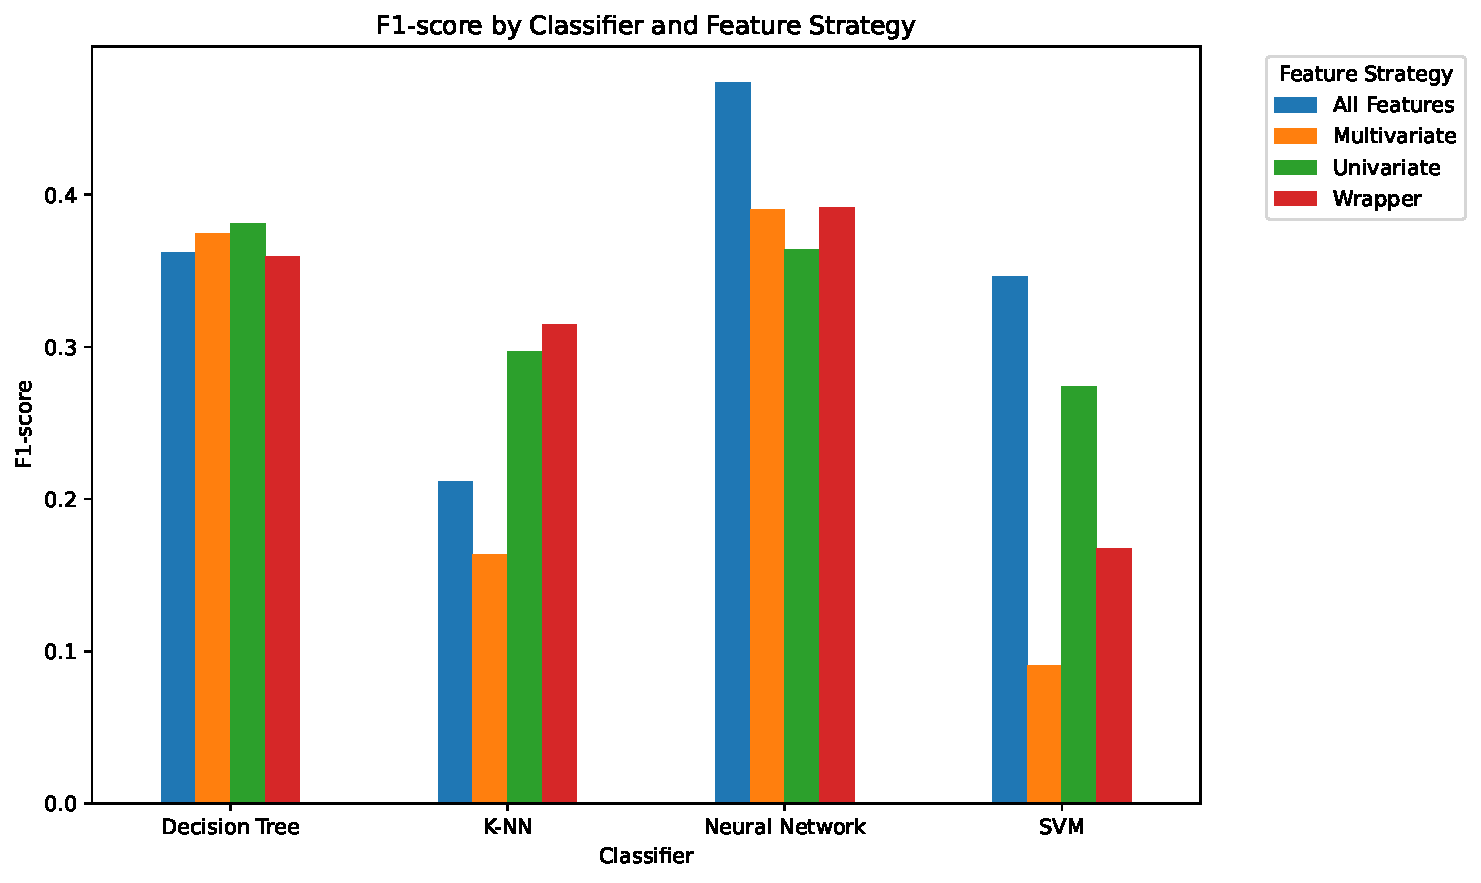
\includegraphics[
        width=0.88\linewidth
    ]{../figures/pa1/f1_comparison.pdf}

    \caption{PA1 mean F1-score by classifier and feature-selection strategy.}
    \label{fig:f1}
\end{figure}

\subsubsection{Selected Variables}

Table~\ref{tab:variables} reports original variables retained by at least two
strategies in the separate full-data interpretation fits. Seven original
variables appear in all three strategies. A categorical variable is counted
as selected when at least one of its dummy features is retained, even when
strategies choose different categories of that variable.

\begin{table}[htbp]
    \centering
    \caption{Agreement between descriptive full-data selections at
    original-variable level. U: univariate; M: multivariate; W: wrapper.}
    \label{tab:variables}
    \small

    \begin{tabular}{lcccc}
\toprule
Original variable & U & M & W & Count \\
\midrule
BusinessTravel & Yes & Yes & Yes & 3 \\
JobInvolvement & Yes & Yes & Yes & 3 \\
JobRole & Yes & Yes & Yes & 3 \\
MaritalStatus & Yes & Yes & Yes & 3 \\
MonthlyIncome & Yes & Yes & Yes & 3 \\
OverTime & Yes & Yes & Yes & 3 \\
StockOptionLevel & Yes & Yes & Yes & 3 \\
Age & Yes & -- & Yes & 2 \\
JobSatisfaction & Yes & Yes & -- & 2 \\
NumCompaniesWorked & -- & Yes & Yes & 2 \\
TotalWorkingYears & Yes & -- & Yes & 2 \\
\bottomrule
\end{tabular}

\end{table}
\subsection{PA2: Probabilistic Classification}
\subsubsection{All Valid Predictors}
Full-feature Logistic Regression obtains the highest F1 among individual probabilistic baselines (0.5373), with accuracy 0.8823, precision 0.7344, recall 0.4259 and specificity 0.9700. It also provides the highest PA2 AUC (0.8375), with Brier 0.1857. Mixed Naive Bayes has the highest recall of all PA2 configurations (0.6453), but lower precision (0.4208), F1 (0.5083), AUC (0.7851) and poorer probability quality (Brier 0.2902). LDA obtains F1 0.4256 and AUC 0.8146; QDA obtains F1 0.3946 and AUC 0.7211.

\subsubsection{Univariate Filter}
Mixed Naive Bayes has the highest F1 within this strategy (0.4600), with recall 0.6033. QDA improves from baseline F1 0.3946 to 0.4240, recall 0.3755 to 0.3924, and AUC 0.7211 to 0.7302, while Brier decreases from 0.2786 to 0.2628. Logistic Regression deteriorates substantially: F1 falls from 0.5373 to 0.3736 and recall from 0.4259 to 0.2708. Thirteen original predictors are retained in all ten folds, including overtime, job level, stock-option level, company tenure, age and monthly income.

\subsubsection{Multivariate Filter}
CFS selects between 3 and 11 original variables per fold (mean 7.8); the separate descriptive full-data fit retains nine. \texttt{JobLevel}, \texttt{OverTime} and \texttt{StockOptionLevel} appear in all ten fold-level subsets, and \texttt{YearsAtCompany} in nine. Mixed Naive Bayes obtains the highest F1 within this strategy (0.3962), with recall 0.3531. The compact subsets therefore lose predictive performance relative to the strongest complete-feature baseline, although its Brier improves from 0.2902 to 0.2386.

\subsubsection{Wrapper}
Logistic Regression obtains the highest F1 among all reduced-feature PA2 configurations (0.4696), with AUC 0.8206 and Brier 0.1976. Mixed Naive Bayes obtains recall 0.4087 and F1 0.4358; QDA obtains F1 0.3848, AUC 0.7165 and Brier 0.2535. Mean selected original-variable counts are 13.1 for Mixed Naive Bayes, 14.6 for Logistic Regression, 13.5 for LDA and 12.9 for QDA. These classifier-specific searches do not outperform the strongest complete-feature baseline.

\subsubsection{Metaclassifiers and Overall Comparison}
Stacking obtains the highest PA2 F1 (0.5394) and lowest Brier (0.1846). Relative to full-feature Logistic Regression, the F1 improvement is marginal, recall is identical (0.4259), and AUC is slightly lower (0.8365 versus 0.8375). AdaBoost obtains F1 0.4676, recall 0.3380 and AUC 0.8314, but its Brier is 0.3773. Bagging obtains F1 0.3407 and recall 0.2362.

Table~\ref{tab:pa2-strategies} summarises the highest-F1 configuration per strategy; Table~\ref{tab:pa2-metrics} identifies the metric-specific leaders. Figure~\ref{fig:pa2-comparison} contrasts F1 with probability-vector error across the evaluated configurations. Rankings use observed cross-validation means and do not establish statistically significant differences.

\begin{table}[htbp]
\centering
\caption{PA2 highest mean F1 configuration per strategy. All scores are ten-fold means; lower Brier is better.}
\label{tab:pa2-strategies}
\small
\setlength{\tabcolsep}{4pt}
\resizebox{\textwidth}{!}{\begin{tabular}{llrrrr}
\toprule
Strategy & Model & Recall & F1 & AUC & Brier \\
\midrule
Metaclassifier & Stacking & 0.425900 & 0.539400 & 0.836500 & 0.184600 \\
All Features & Logistic Regression & 0.425900 & 0.537300 & 0.837500 & 0.185700 \\
Wrapper & Logistic Regression & 0.355100 & 0.469600 & 0.820600 & 0.197600 \\
Univariate & Mixed Naive Bayes & 0.603300 & 0.460000 & 0.763300 & 0.319000 \\
Multivariate & Mixed Naive Bayes & 0.353100 & 0.396200 & 0.761600 & 0.238600 \\
\bottomrule
\end{tabular}
}
\end{table}

\begin{table}[htbp]
\centering
\caption{PA2 leading configurations by objective metric.}
\label{tab:pa2-metrics}
\small
\setlength{\tabcolsep}{4pt}
\begin{tabular}{lllr}
\toprule
Metric & Strategy & Model & Value \\
\midrule
F1 & Metaclassifier & Stacking & 0.539400 \\
Recall & All Features & Mixed Naive Bayes & 0.645300 \\
AUC & All Features & Logistic Regression & 0.837500 \\
Brier & Metaclassifier & Stacking & 0.184600 \\
\bottomrule
\end{tabular}

\end{table}

\begin{figure}[htbp]
\centering
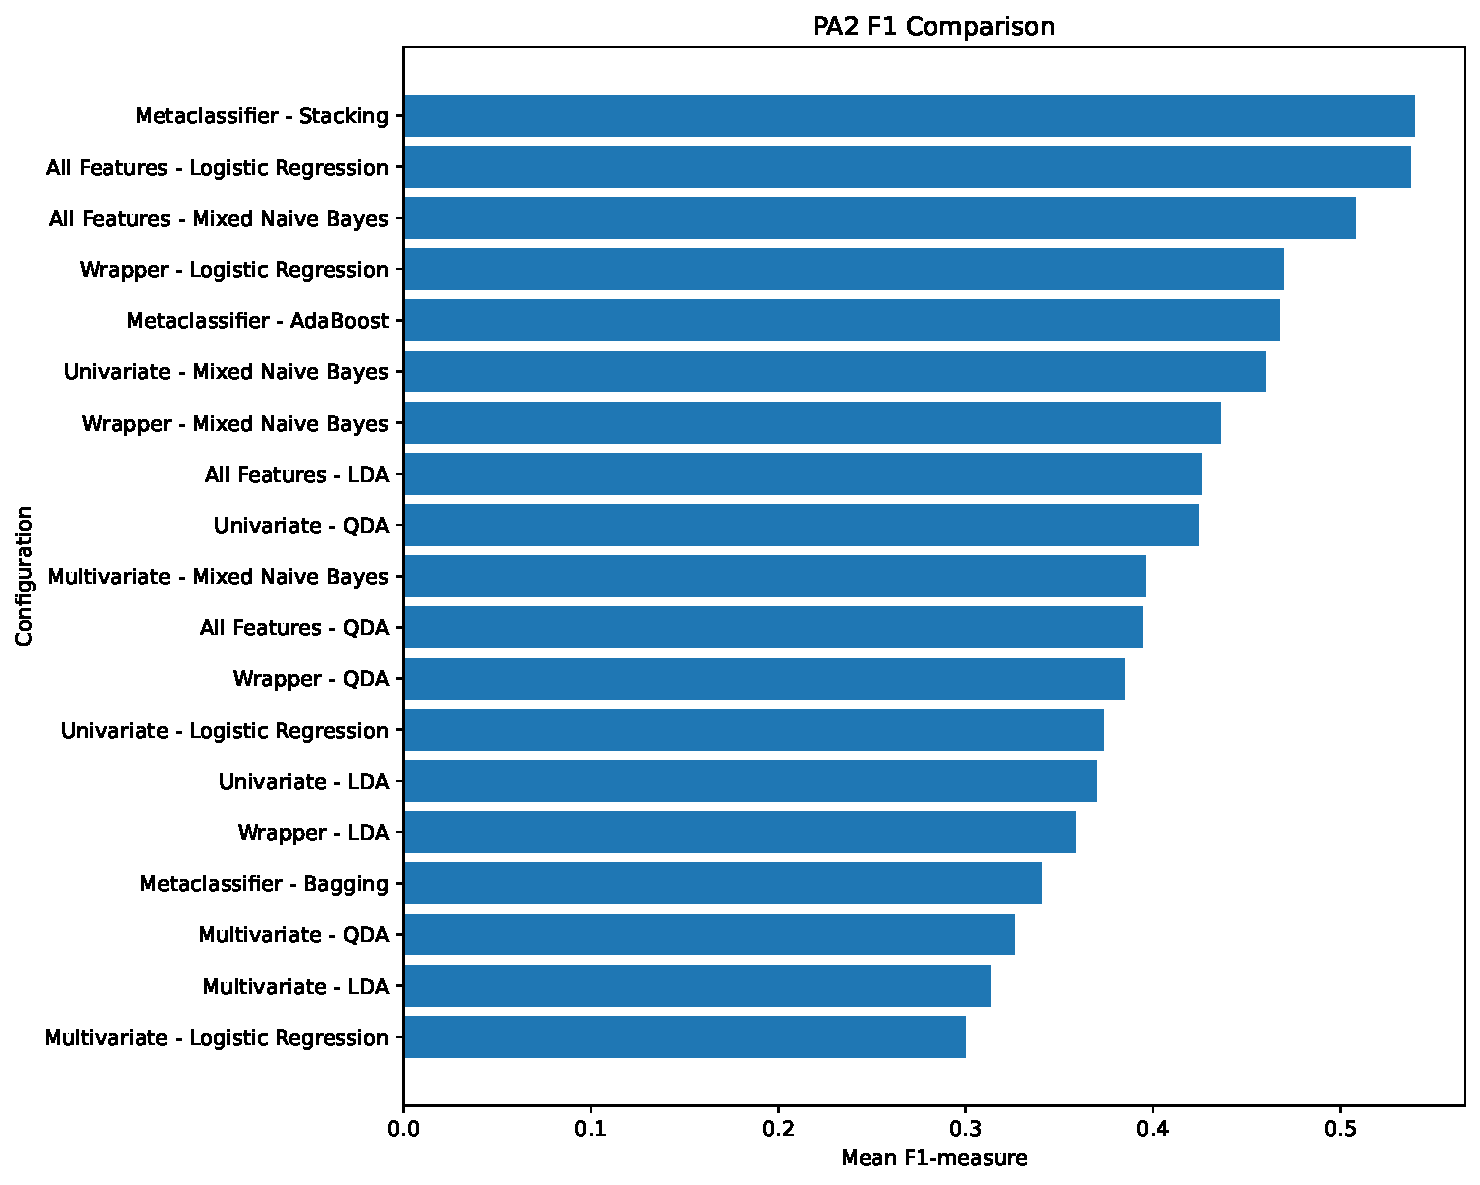
\includegraphics[width=0.76\linewidth]{../figures/pa2/f1_comparison.pdf}
\par\medskip
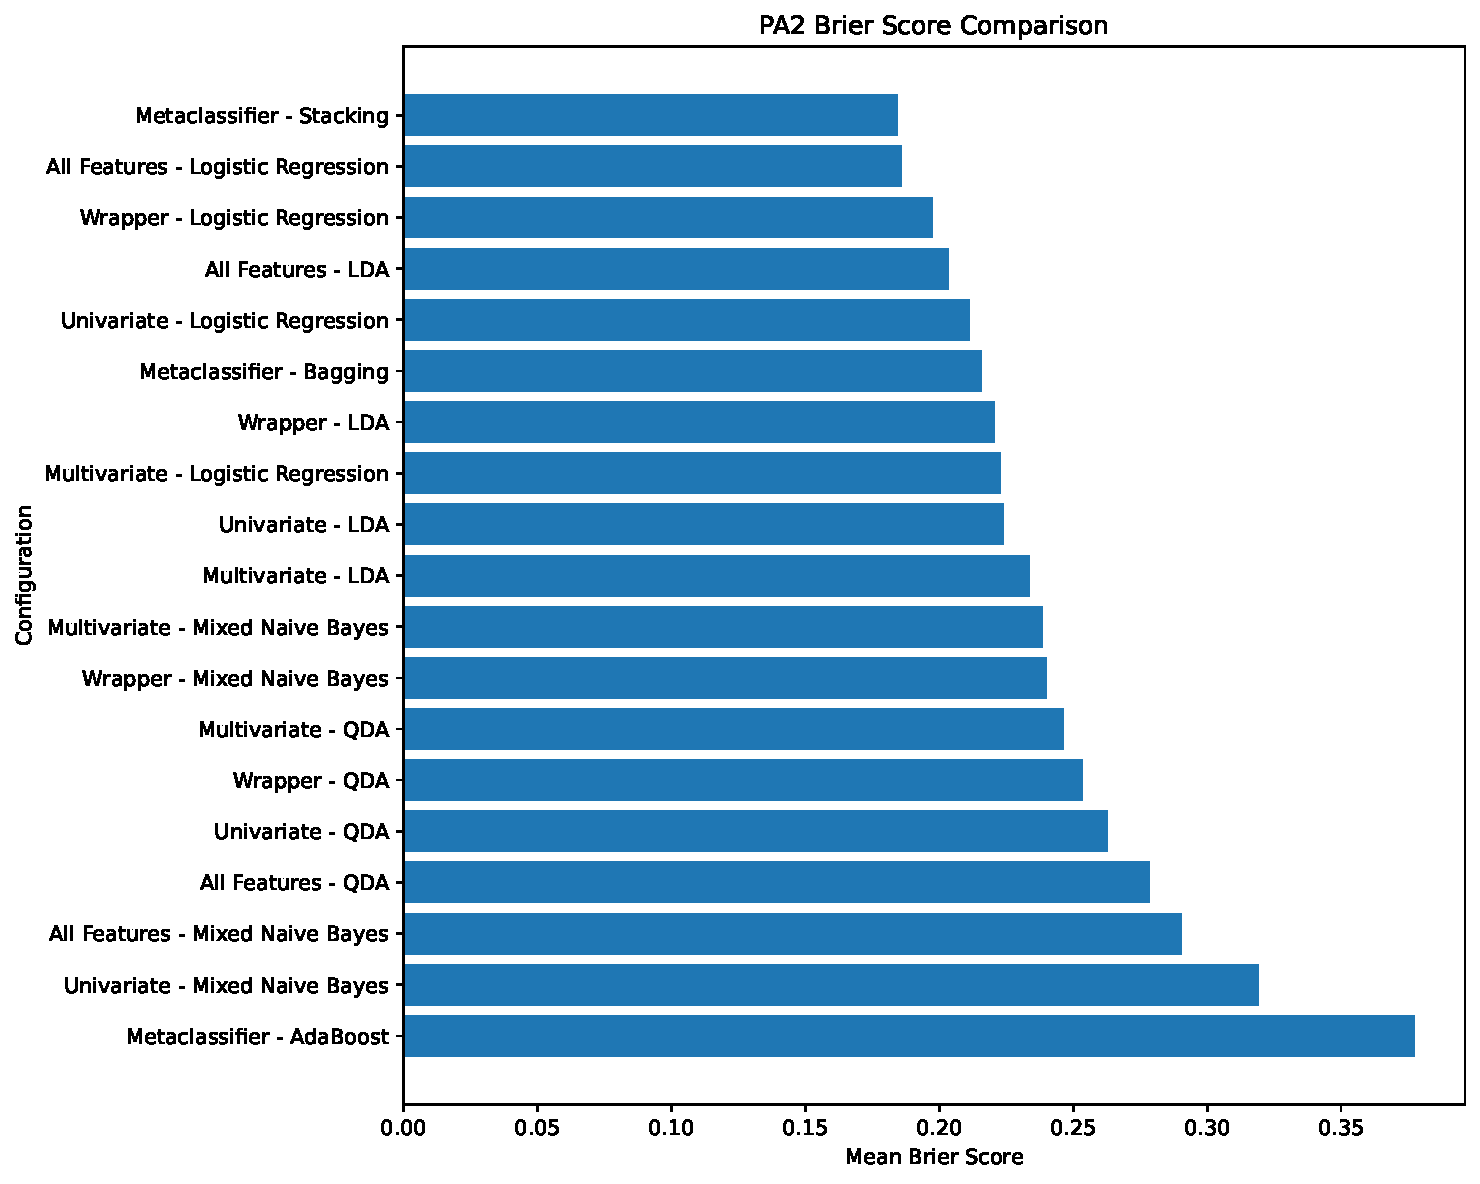
\includegraphics[width=0.76\linewidth]{../figures/pa2/brier_comparison.pdf}
\caption{PA2 mean F1 (top) and full class-probability-vector Brier score (bottom). Higher F1 and lower Brier are preferable.}
\label{fig:pa2-comparison}
\end{figure}
\clearpage
